%000000000000000000000000000000000000000000000000000000000000000000000000000000
\subsection{Package sequenziatore::server::presenter}
\begin{figure}[H] \centering 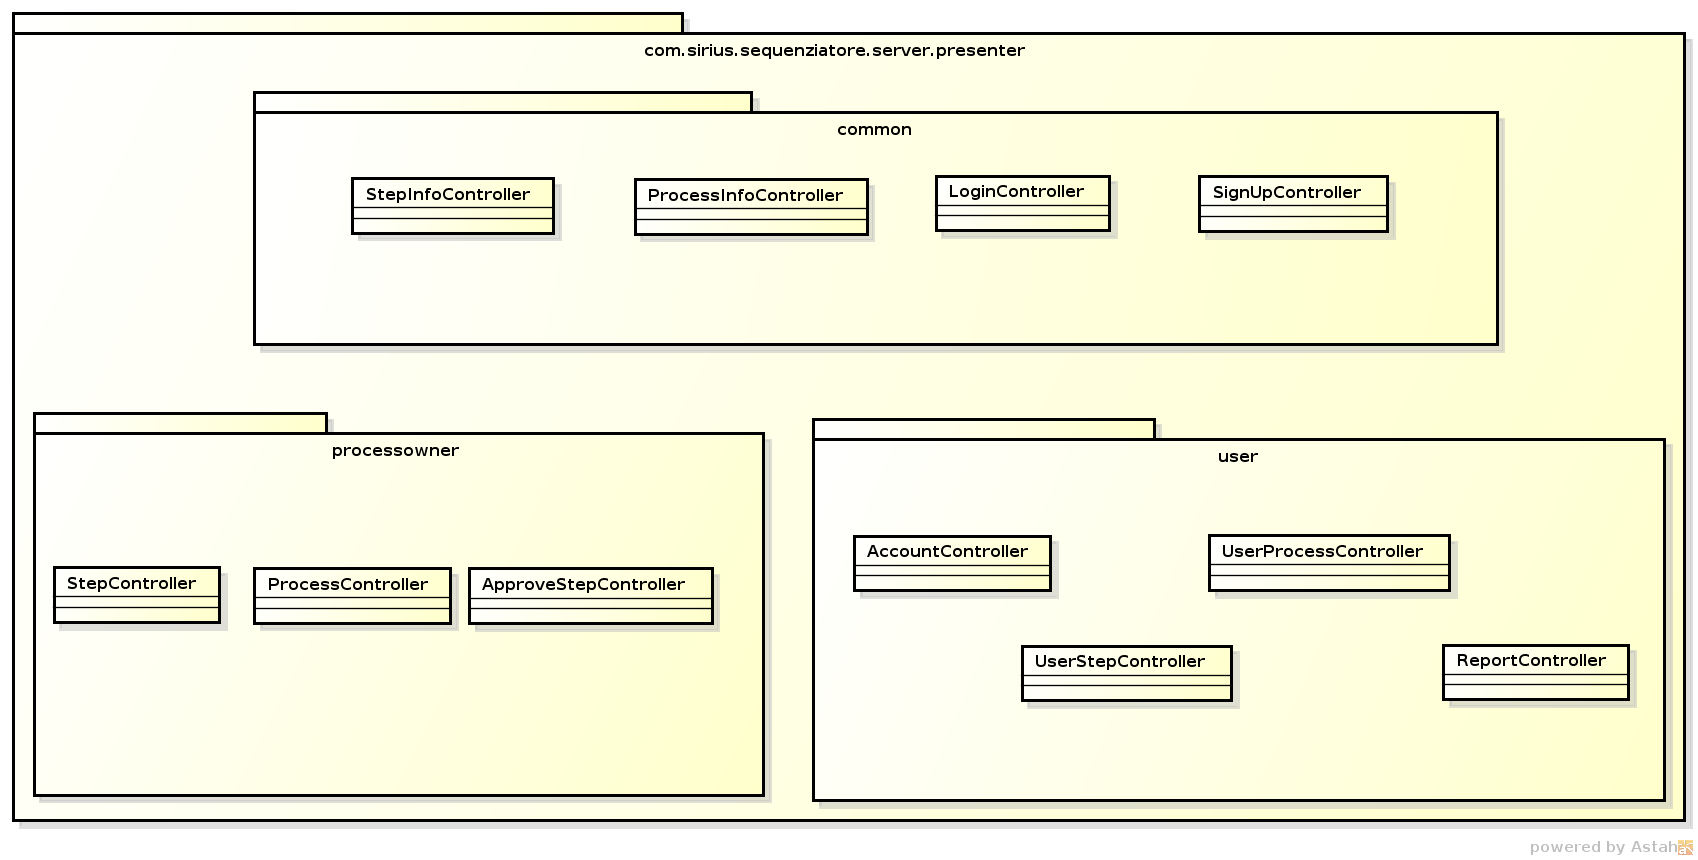
\includegraphics[width=%
\textwidth]
{./pack/ClassiServerSoloPresenter.png} \caption{Diagramma presenter server}
\end{figure}
%000000000000000000000000000000000000000000000000000000000000000000000000000000000000000000000000000000000%
\subsubsection{Package sequenziatore::server::presenter::user}
\paragraph{AccountController}
	\begin{itemize}
		\item \textbf{Nome:} \texttt{AccountController};
		\item \textbf{Package:} sequenziatore::server::presenter::user
		\item \textbf{Descrizione:} classe che permette la modifica dei dati di un utente come password o altre informazioni e il controllo del \textit{log in} di un utente;
		\item \textbf{Relazione con altre componenti:} la classe richiama i metodi della classe:
		\begin{itemize}
			\item sequenziatore::server::model::IDataAccessObject;
		\end{itemize}
	\end{itemize}
%-----------------------------------------------------------------------------------------------%
\paragraph{UserProcessController}
	\begin{itemize}
		\item \textbf{Nome:} \texttt{UserProcessController};
		\item \textbf{Package:} sequenziatore::server::presenter::user
		\item \textbf{Descrizione:} classe che restituisce all' utente i dati di uno o più processi, può inoltre permettere l' inoltro della richiesta di un utente a iscriversi o disiscriversi a un processo;
		\item \textbf{Relazione con altre componenti:} la classe richiama i metodi della classe:
		\begin{itemize}
			\item sequenziatore::server::model::IDataAccessObject;
		\end{itemize}
	\end{itemize}
%-----------------------------------------------------------------------------------------------%
\paragraph{UserStepController}
	\begin{itemize}
		\item \textbf{Nome:} \texttt{UserStepController};
		\item \textbf{Package:} sequenziatore::server::presenter::user
		\item \textbf{Descrizione:} Gestisce l' esecuzione di un passo da parte di un utente inoltrando la richiesta di inserire i dati nel \textit{database} e in caso sia richiesto, notifica l' amministratore che deve controllare se il passo è stato completato, inoltre è incaricato di restituire i dati di un passo quando richiesto da un utente;
		\item \textbf{Relazione con altre componenti:} la classe richiama i metodi della classe:
		\begin{itemize}
			\item sequenziatore::server::model::IDataAccessObject;
		\end{itemize}
	\end{itemize}
%-----------------------------------------------------------------------------------------------%
\paragraph{Report}
	\begin{itemize}
		\item \textbf{Nome:} \texttt{Report};
		\item \textbf{Package:} sequenziatore::server::presenter::user
		\item \textbf{Descrizione:} Classe che genera il report dell' utente riferito al processo richiesto;
		\item \textbf{Relazione con altre componenti:} la classe implementa l' interfaccia sequenziatore::server::presenter::iuser::IReport e richiama i metodi delle classi:
		\begin{itemize}
			\item sequenziatore::server::model::IDataAccessObject;
		\end{itemize}
	\end{itemize}
%-----------------------------------------------------------------------------------------------%